\section{Auswertung}
\label{sec:Auswertung}

\subsection{Brennweitenbestimmung durch Messung von Gegenstands- und Bildweite}

In \ref{tab:brenn} sind die Werte für die Positionen des Gegenstandes $P_L$ und die Position des Schirms $P_S$ eingetragen.
Durch diese Werte lässt sich mit
\begin{equation}
  g=P_L-P_G
\end{equation}
die Gegenstandsweite ausrechnen.
Für die Bildweite gilt
\begin{equation}
  b=P_S-P_L
\end{equation}.
Auch die Größe des Bildes $B$ wurde gemessen.
Mit der Formel \ref{eqn:abbildung1} wird $V_1$ und mit \ref{eqn:abbildung1} wird $V_2$ berechnet.
Auch diese Werte, sowie die Differenz zwischen beiden, werden in Tabelle \ref{tab:brenn} hinzugefügt.
Die Brennweite der Linse wird mit \ref{eqn:brenn2} ausgerechnet und ebenfalls in die Tabelle eingetragen.

\begin{table}
  \caption{Aufgeführt sind hier die gemessene Position der Linse, sowie die davon abhängige Position des Schirms um ein scharfes Bild zu erhalten.
  Zudem wurden aus diesen Werten Ggenstands- und Bildweite berechnet. 
  Dazu wurde die Größe des Bildes gemessen und einerseits mit den gemessenen Größen und andererseits mit Bild- und Gegenstandsweite der Abbildungsmaßstab berechnet.
  $\delta V$ ist die Differenz davon. Die Ungenauigkeit dieser Werte beträgt $\pm \qty{0.1}{\centi\meter}}$.

  \label{tab:brenn}
  \centering
  \begin{tblr}{
    colspec{S[table-format=2.0] S[table-format=2.1] S[table-format=2.0] S[table-format=2.1] S[table-format=1.1]};
    row{1}={guard, mode=math};
    }
    \toprule
    P_L \mathbin{/} \unit{\centi\meter} & P_S \mathbin{/} \unit{\centi\meter} & g \mathbin{/} \unit{\centi\meter} & b \mathbin{/} \unit{\centi\meter}
     & B \mathbin{/} \unit{\centi\meter} & V_1 \mathbin \unit{\centi\meter} &\\
    \midrule
    40   &   65.9  &  15  & 25.9  &  5.0\\
    45   &   64.0  &  20  & 19.0  &  2.9\\
    50   &   66.5  &  25  & 16.5  &  2.2\\
    55   &   70.2  &  30  & 15.2  &  1.8\\
    60   &   74.6  &  35  & 14.6  &  1.0\\
    65   &   78.8  &  40  & 13.8  &  0.8\\
    70   &   83.6  &  45  & 13.6  &  0.6\\
    75   &   88.3  &  50  & 13.3  &  0.5\\
    80   &   93.0  &  55  & 13.0  &  0.4\\
    85   &   97.7  &  60  & 12.7  &  0.3\\
  \end{tblr}

\end{table}

\begin{figure}[H]
  \centering
  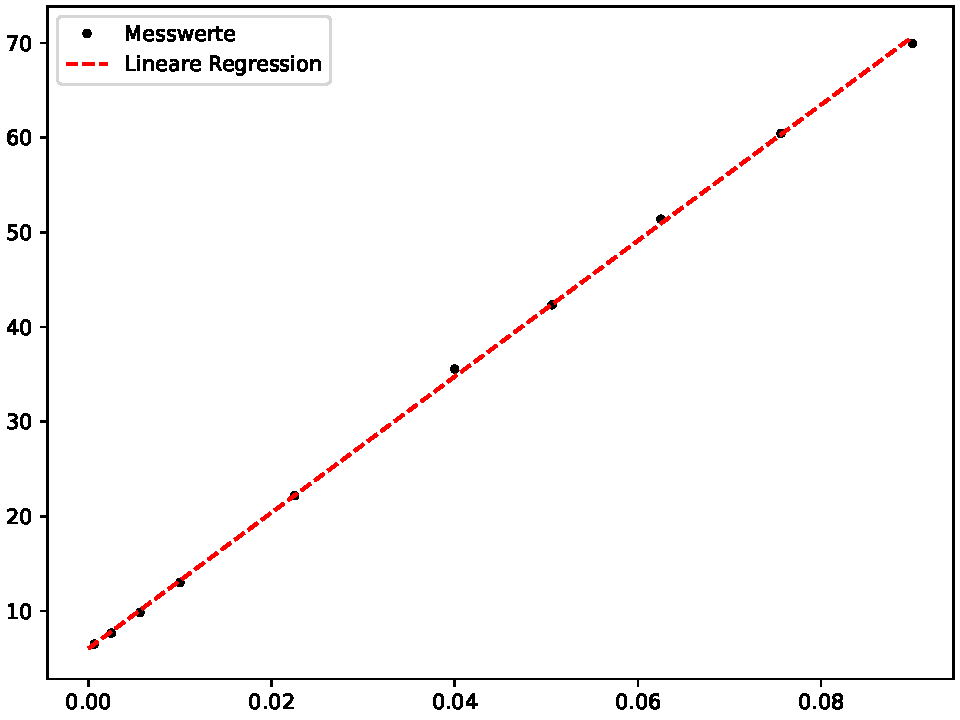
\includegraphics{plot.pdf}
  \caption{Abgebildet sind die Werte der Bildweite auf der y-Achse und die der Gegenstandsweite auf der x-Achse.}
  \label{fig:brenn}
\end{figure}

\subsection{Brennweitenbestimmung mit der Methode von Bessel}

\begin{table}
  \caption{Messwerte ohne einen Farbfilter.}
  \label{tab:bessel}
  \centering
  \begin{tblr}{
    colspec={S[table-format=1.1] S[table-format=1.1] S[table-format=1.1] S[table-format=1.1]};
    row{1}={guard, mode=maths};
  }
  \toprule
  P_{L1} \mathbin{/} \unit{\centi\meter}  & P_{L2} \mathbin{/} \unit{\centi\meter} & P_S \mathbin{/} \unit{\centi\meter} \\
  \midrule
  38.5  &  54.6   &  70     \\
  37    &  60.7   &  75     \\
  36.6  &  66.4   &  80     \\
  36.1  &  71.6   &  85     \\
  35.9  &  76.7   &  90     \\
  35.8  &  82.1   &  95     \\
  35.8  &  87.2   &  100    \\
  35.4  &  92.5   &  105    \\
  35.2  &  97.5   &  110    \\
  35.2  &  102.7  &  115    \\  
  \bottomrule
  \end{tblr}
\end{table}
%\begin{table}
%  \centering
%  \caption{Eine Beispieltabelle mit Messdaten.}
%  \label{tab:tabelle}
%  \sisetup{table-format=1.1, per-mode=reciprocal}
%  \begin{tblr}{
%      colspec = {S[table-format=3.0] S[table-format=2.1] S},
%      row{1} = {guard, mode=math},
%      vline{4} = {2}{-}{text=\clap{$\pm$}},
%    }
%    \toprule
%    U \mathbin{/} \unit{\volt} & I \mathbin{/} \unit{\micro\ampere} & \SetCell[c=2]{c} N \mathbin{/} \unit{\per\second} & \\
%    \midrule
%    360 & 0.1 & 98.3 & 0.9 \\
%    400 & 0.2 & 99.8 & 1.0 \\
%    420 & 0.2 & 99.1 & 0.9 \\
%    \bottomrule
%  \end{tblr}
%\end{table}

Siehe \autoref{fig:plot} und \autoref{tab:tabelle}!


\subsection{Brennweitenbestimmung mit der Methode von Abbe}

